\documentclass{beamer}
\usetheme{metropolis}           % Use metropolis theme
\metroset{numbering=fraction}
\usepackage[T2A]{fontenc}
\usepackage[utf8]{inputenc}
\usepackage[english,russian]{babel}

\title{Декларативное программирование}
\subtitle{Семинар №8, группа 22215}
\author{Завьялов А.А.}
\date{24 октября 2022 г.}
\institute{Кафедра систем информатики ФИТ НГУ}
\begin{document}
  \maketitle
  \section{Два вида полиморфизма в Haskell}
  \section{Классы типов}
  \begin{frame}{Иерархия некоторых стандартных классов типов}
      \begin{figure}
          \centering
          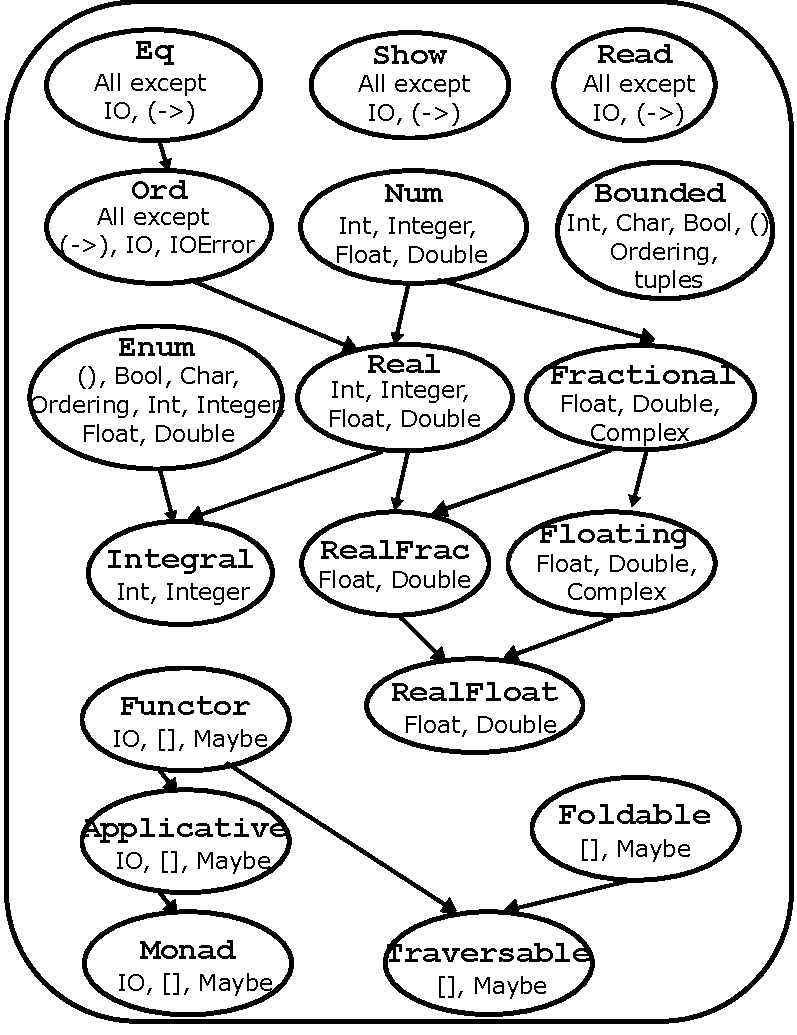
\includegraphics[scale=0.45]{media/base-classes.pdf}
      \end{figure}
  \end{frame}
  \section{Очевидно полезные классы типов}
  \section{Полугруппы, моноиды}
  \section{Функторы}
  \begin{frame}{Что почитать?}
      \begin{itemize}
          \item Введение в теорию языков программирования --- Ж.~Довек, Ж-Ж. Леви
          \item Типы в языках программирования --- Бенджамин Пирс (TaPL)
          \item \url{https://wiki.haskell.org/Typeclassopedia}
      \end{itemize}
  \end{frame}
  \section{Q\&A}
\end{document}